\thispagestyle{empty}

\begin{center}
{\heiti\fontsize{18bp}{18bp}\selectfont\bfseries 五一数学建模竞赛}\par
\vspace{5mm}
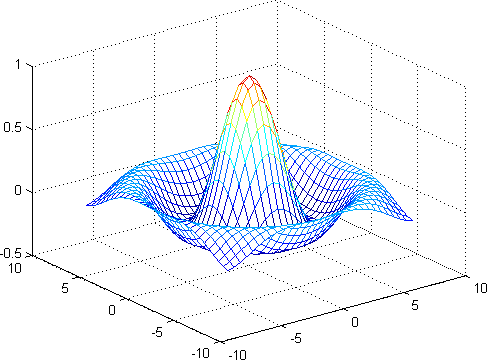
\includegraphics[width=32mm]{figures/image1.png}\par
\vspace{6mm}
{\heiti\sanhao[1]\bfseries 题目：基于阶段归一化残差融合的边坡变形预测与预警模型}\par
\end{center}

\vspace{4mm}
\noindent{\heiti 关键词：}Huber稳健校准；复合证据变点；Kalman补全；阶段归一化基线；逆速度预警

\vspace{3mm}
\noindent{\heiti 摘要：}

针对边坡监测数据存在传感器尺度差异、异常缺失、阶段性变形和多源扰动耦合等问题，本文建立“鲁棒校准--复合证据分段--变量专属异常识别--阶段归一化残差预测--速度预警闭环”的一体化模型。模型以可解释的阶段变形骨架为主线，将机器学习限制在残差修正和贡献排序中，并用多模型对照、bootstrap置信区间、窗口敏感性和消融实验构造稳健性证据。

问题一采用Huber稳健仿射校准，将A传感器映射到B传感器基准；与OLS、Theil--Sen和RANSAC对照后，Huber模型交叉验证MAE为1.289 mm，5个待校正值为5.762、15.809、73.836、108.415和147.311 mm。问题二以Hampel去尖峰后的6 h滚动中位速度为主证据，并结合位移趋势和持续加速度，确定两阶段转换主节点为第8108号和第9501号。问题三按变量性质区分连续状态量与稀疏驱动量，补齐后无缺失且非负变量无负值，共识别单变量异常63个、共同异常17个；HistGBDT验证集$R^2$为0.877，孔隙水压力和深部位移是最稳定主控因素。问题四采用阶段归一化基线与扰动残差模型，“阶段基线+GBDT残差”的时间块交叉验证RMSE为2.142 mm，实验集5个指定时刻预测值为5.163、30.767、60.259、383.185和383.697 mm，并给出95\%预测区间。问题五枚举全部六选五变量组合，最终选择降雨量、孔隙水压力、微震事件数、爆破点距离和单段最大药量；预警采用6 h平滑速度，设置2.980、6.418和9.949 mm/h三级阈值，并叠加持续时间、多源扰动增强和逆速度下降趋势，形成可复现的工程预警机制。

\clearpage
